\documentclass[multi,tikz,crop=false,class=article]{standalone}
\onlyifstandalone{\usepackage{hyperref}
\usepackage{cleveref}
\usepackage[disable]{todonotes}
\presetkeys{todonotes}{inline, noline}{}
\usepackage{caption}
\usepackage{subcaption}
\usepackage{amsfonts}
\usepackage{theorem}
\usepackage{algorithm}
\usepackage{algpseudocode}
\theoremstyle{plain}
\theorembodyfont{\slshape}
\newtheorem{definition}{Definition}[section]
\usepackage{algorithm}
\usepackage{algpseudocode}
\usepackage{amsmath}
\usepackage{mathtools}
\usepackage{tikz}

\usetikzlibrary{automata,arrows}

%\DeclareCaptionType{algorithm}
\algdef{SE}[DOWHILE]{Do}{doWhile}{\algorithmicdo}[1]{\algorithmicwhile\ #1}%

% Math macros
\newcommand{\concat}{\cdot}
\newcommand{\bool}{\ensuremath{\mathbb{B}}}
\newcommand{\lang}{\ensuremath{\mathcal{L}}}
\newcommand{\dstar}[2]{\ensuremath{\delta^*(#1,#2)}}
\newcommand{\exec}[2]{\ensuremath{#1[#2]}}
\newcommand{\access}[2]{\ensuremath{#1^{-1}[#2]}}
\newcommand{\nero}{\ensuremath{\equiv}}
\newcommand{\eqclass}[2]{\ensuremath{[#1]_{#2}}}
\newcommand{\mq}{\ensuremath{\mathsf{member}}}
\newcommand{\eq}{\ensuremath{\mathsf{equiv}}}
\newcommand{\row}{\ensuremath{\mathsf{row}}}
\newcommand{\sift}{\ensuremath{\mathsf{sift}}}
%%% Local Variables:
%%% mode: latex
%%% TeX-master: t
%%% End:
}
\usepackage{amsmath}
\DeclareMathOperator{\row}{row}
\usetikzlibrary{automata,arrows}

\begin{document}
\section{Fundamental Theory}
\label{sec:fundamental-theory}
This part introduces the theory fundamental to active state machine learning:
the notion of Nerode-equivalence, and the original learning algorithm due to
Angluin called $L^*$. Before this, an explanation of the notation used
throughout the article is in order. First, the assumed definition of a DFA is
introduced.

\begin{definition}[Deterministic Finite Automaton]\label{def:dfa}
  A DFA $M$ is a 5-tuple $(Q, q_0, \Sigma, \delta, F)$ where $Q$ is the set of
  states, $q_0$ the initial state, $\Sigma$ the input alphabet, $\delta$ the
  transition function, and $F$ the set of accepting states.
\end{definition}

Define $\Sigma^*$ to be all of the words constructed from the input alphabet
$\Sigma$. Furthermore, $\epsilon$ represents the empty word. Note that by
definition it holds that $\epsilon \in \Sigma^*$. The concatenation operator is
denoted $v \concat w$ for two strings in $\Sigma^*$ or elements in the input
alphabet $\Sigma$.

For some word $w \in \Sigma^*$, let $\dstar{q}{w}$ denote the state reached by
executing $w$ from state $q$. Furthermore, denote $\exec{M}{w} = \dstar{q_0}{w}$
to be the state reached by executing $w$ from the initial state $q_0$, as used
by Kearns and Vazirani\cite{Kearns94}. Lastly, let $\lang_M$ denote the regular
language accepted by $M$; that is $\lang_M = \{ w \mid \exec{M}{w} \in F \}$.

Below two definitions are given which together provide the necessary background
theory of the field of active state machine learning.

\begin{definition}[Distinguishing Extension]\label{def:dist-ext}
  Let $\lang$ be a language over some alphabet $\Sigma$, and let $v$, $w$ and
  $z$ be words in $\Sigma^*$. Then $z$ is a \textit{distinguishing extension}
  for $v$ and $w$ if and only if \textit{exactly one} of $v \concat z$ and
  $w \concat z$ is in $\lang$.
\end{definition}
\begin{definition}[Nerode-equivalence]\label{def:nerode-eq}
  For some language $\lang$ over an alphabet $\Sigma$, define two words
  $v,w \in \Sigma^*$ to be \textit{Nerode-equivalent} with respect to
  $\lang$ if and only if there is no distinguishing extension $z$ for $v$
  and $w$. We write $v \nero_\lang w$ if $v$ and $w$ are Nerode-equivalent.

  Let $\eqclass{w}{\lang}$ denote the \textit{equivalence class} of $w$, such
  that for any word $v$ in $\eqclass{w}{\lang}$ it holds that $v \nero_\lang
  w$. Lastly, let $\nero_\lang$ be the set of all equivalence classes of
  $\lang$. For convenience, denote $\nero_M$ to be the same set for some DFA
  $M$.
\end{definition}

%TODO: Cite Myhill and Nerode
From the above \cref{def:nerode-eq}, the Myhill-Nerode theorem makes a strong
statement: a language $\lang$ is regular if and only if the set of equivalence
classes $\nero_\lang$ is a finite set. Indeed, this theorem is stronger than the
pumping lemma for regular languages, which can only prove that a language is
\textit{not} regular.

%TODO: Cite Hopcroft and Ullman
According to Hopcroft and Ullman, each regular language $\lang$ has a minimal
DFA $M$ which accepts $\lang$. The amount of states of $M$ is precisely equal to
the amount of equivalence classes $\nero_\lang$, thus there is a one-to-one
correspondence between each equivalence class and each state of $M$.

Thus, from a set of equivalence classes $\nero_M$, $M$ can be constructed as
follows. Let $\nero_M$ represent the set of states of $M$. For each state
$\eqclass{w}{\lang_M}$ and for each $\sigma \in \Sigma$, an outgoing transition
can be constructed to the state $\eqclass{w\concat\sigma}{\lang_M}$. The initial
state would be represented by the equivalence class
$\eqclass{\epsilon}{\lang_M}$. Lastly, a state $\eqclass{w}{\lang_M}$ is an
accepting state if and only if $\eqclass{w}{\lang_M} \subseteq \lang_M$.

\subsection{Key Principle of Active Learning}
\label{sec:key-principle-active}
In active state machine learning, the goal is to learn an unknown DFA $M$ (the
\textit{target}), which is assumed to be minimal. The key principle of all
active state machine learning algorithms is to progressively refine a hypothesis
DFA $\hat M$ until it equals $M$.

Put in terms of equivalence classes, a learning algorithm progressively refines
a set of equivalence classes $\nero_{\hat M}$, until it eventually converges to
the set of equivalence classes $\nero_M$ of the target.

Any active learning algorithm has access to a so-called \textit{minimally
  adequate teacher} (MAT) which can answer two types of queries about the
target:

\begin{description}
\item[Membership Query] Given a word, answers ``yes'' or ``no'' depending on
  whether it is accepted by the target $M$ or not.
\item[Equivalence Query] Given a hypothesis DFA $\hat M$, answers ``yes'' if
  $\hat M$ equals $M$, in which case the algorithm is finished. If the
  hypothesis is not equal, it provides a counterexample $\gamma$. The
  counterexample can be used to further refine $\nero_{\hat M}$, since $\gamma$
  is an example of an incorrect equivalence class.
\end{description}

Note that for the equivalence query, the hypothesis can be constructed in a
manner similar to the construction described in the previous section.

Furthermore, note that the algorithm is guaranteed to converge to the target DFA
$M$, since $\nero_M$ must be finite according to the Myhill-Nerode theorem, and
the learning algorithms that will be discussed guarantee progress after every
equivalence query.
% TODOs:
% Done: Explain connection minimal DFA <-> equivalence classes
% Explain principle of active state machine learning: refining a set of
%   equivalence classes until it equals the set of equivalence classes of the
%   target DFA.
% Cite Myhill & Nerode and Hopcroft & Ullman
% Done: Explain membership and equivalence queries and relationship with key
%   principles.

\subsection{An Algorithm for Learning DFAs}
Angluin defines the $L^*$ algorithm for learning regular sets\cite{Angluin87}.
The goal of the algorithm is to discover a model that corresponds to the regular
set (`the target').

The target is said to contain only \textit{words}, where each word consists
of the concatenation of zero or more items from a certain set of of symbols
called the input alphabet $\Sigma$.

\subsubsection{Data structure}
\label{sec:data-structure}
The algorithm keeps track of a set of \textit{access strings} $S$ and a set of
\textit{distinguishing extensions} $E$. The answers to the queries are stored in
a two-dimensional table called an observation table. The columns of this table
are headered by the items of $E$. The rows are split into two parts. The rows of
the upper and lower parts are headered by items from $S$ and $S \concat \Sigma$
respectively, where `$\concat$' is the concatenation operator.

% not quite happy with this phrasing yet.. 
Rows in the observation table correspond to state candidates for the hypothesis.
Two state candidates are considered to represent the same state if they react
identically under the same input (i.e. if the corresponding rows have the same
values under all columns). Consider a cell at the row $x$ labelled by access
string $s$ and column $e$. The value at column $e$ represents whether applying
the string $e$ from the state corresponding to $x$ results in an accepting
state. Equivalently, this can be interpreted to mean whether applying $s \concat
e$ from the initial state results in an accepting state.

\subsubsection {The algorithm}
\todo{Introduce equivalence classes}

The algorithm begins by initializing $S$ and $E$ to $\{\epsilon\}$ (where
$\epsilon$ is the empty access string) and performing membership queries to fill
in the observation table. After the initialization is done, the main loop runs
until a hypothesis matching the target is found. The main loop is split up into
two phases. The first phase is repeated until a closed and consistent model is
found.

A model is called inconsistent if and only if the observation table contains
distinct rows with identical values under $E$ (i.e. the rows appear to represent
the same state), but inputting some $\sigma \in \Sigma$ results in rows with
different values for some $e \in E$. Thus if a model is found to be
inconsistent, feeding the input $\sigma \concat e$ results in different states,
and so $\sigma \concat e$ is discovered to be a distinguishing experiment.
Therefore, $\sigma \concat e$ is added to $E$, making the two rows in $S$
distinct under the columns of $E$, thus removing the inconsistency. New
membership queries are performed in order to fill in the blank cells in the
table.

A model is considered to be closed if $S \concat \Sigma$ does not contain any
states that are not in $S$. If there is a row $x$ in $S \concat \Sigma$ that is
not in $S$, then it is unknown how $x$ reacts to $\Sigma$. This means that the
current hypothesis of the state machine does not describe what happens in state
$x \concat \Sigma$. To address this problem, $x$ is moved to $S$ and for each $y
\in x \concat \Sigma$, a row labelled by $y$ is added to the lower part of the
observation table. The values in the new rows in the lower part of the table are
set by executing the required membership queries.

In the second phase of the algorithm, the observation table is both closed and
consistent. The algorithm uses the observation table to construct a hypothesis.
Each row from the table represents a candidate state, but since the table can
contain duplicate rows, multiple rows (and therefore, candidate states) can map
to the same state. The hypothesis contains one state for each unique row in the
table. Let $f(x)$ denote the state in the hypothesis corresponding to the access
string $x$. The initial state in the hypothesis is the state $f(\sigma)$. All
states corresponding to rows that have a $1$ under the column $\epsilon$ are
accepting states. For each unique row in the upper part of the table, let $s \in
S$ denote the label corresponding to the row. Then the hypothesis contains a
transition for each $\sigma \in \Sigma$ from $f(s)$ to $f(s \concat \sigma)$,
constrained by $\sigma$. Note that since the observation table is closed, the
upper part of the table contains all unique rows, so $\row(s \concat \sigma)$
can always be looked up in the lower part of the table.

Once the hypothesis is constructed, the equivalence query is executed upon it.
If the hypothesis matches the target then the algorithm stops. If instead a
counterexample is replied, the counterexample and all of its prefixes are added
to $S$, after which $S \concat \Sigma$ is updated and the algorithm moves back
to phase 1.

\subsubsection {Example run}

Suppose $L^*$ is used to learn the target DFA $U$ of figure \ref{fig:target}.
The input alphabet for this DFA is $\Sigma = \{a, b\}. $ $L^*$ initializes $S$
and $E$ to $\{\epsilon\}$, and performs three membership queries to build the
initial observation table of table \ref{tbl:observation_1}.

\begin{figure}[t]
\centering
\begin{subfigure}[b]{.4\textwidth}
\centering
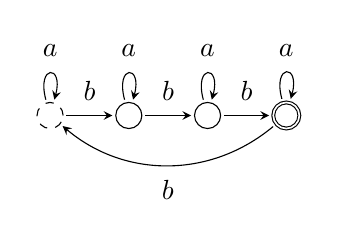
\begin{tikzpicture}
  [bend angle=40,every node/.style={draw,circle}]

  \tikzstyle{initial} = [dashed]

  \node[initial]   (1) at (1,0) {};
  \node            (2) at (2,0) {};
  \node            (3) at (3,0) {};
  \node[accepting] (4) at (4,0) {};

  \path[->, >=stealth, shorten > = 1pt, shorten < = 1pt]
        (1) edge              node[auto,draw=none] {$b$} (2) 
        (2) edge              node[auto,draw=none] {$b$} (3)
        (3) edge              node[auto,draw=none] {$b$} (4)
        (1) edge [loop above] node[auto,draw=none] {$a$} (1)
        (2) edge [loop above] node[auto,draw=none] {$a$} (2)
        (3) edge [loop above] node[auto,draw=none] {$a$} (3)
        (4) edge [loop above] node[auto,draw=none] {$a$} (4)
        (4) edge [bend left]  node[auto,draw=none] {$b$} (1);
\end{tikzpicture}
\caption{The target} \label{fig:target}
\end{subfigure}
\hfill
\begin{subfigure}[b]{0.4\textwidth}
\centering
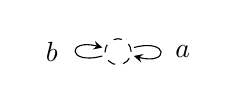
\begin{tikzpicture}
  [bend angle=40,every node/.style={draw,circle}]

  \tikzstyle{initial} = [dashed]

  \node[initial]   (1) at (1,0) {};

  \path[->, >=stealth, shorten > = 1pt, shorten < = 1pt]
        (1) edge [loop right] node[auto,draw=none] {$a$} (2) 
        (1) edge [loop left]  node[auto,draw=none] {$b$} (2);
\end{tikzpicture}
\caption{First hypothesis} \label{fig:hypoth_1}
\end{subfigure}
\caption{Automata}
\end{figure}


\begin{table}
\centering

\begin{subtable}[h]{.23\textwidth}
\centering
\begin{tabular}{ | l || c | }
\hline
           & $\epsilon$ \\ \hline \hline
$\epsilon$ & $0$        \\ \hline \hline
$a$        & $0$        \\
$b$        & $0$        \\
\hline
\end{tabular}
\caption{} \label{tbl:observation_1}
\end{subtable}
%
%
\hfill
\begin{subtable}[h]{.23\textwidth}
\centering
\begin{tabular}{ | l || c | }
\hline
           & $\epsilon$ \\ \hline \hline
$\epsilon$ & $0$        \\ 
$b$        & $0$        \\ 
$bb$       & $0$        \\ 
$bbb$      & $1$        \\ \hline \hline
$a$        & $0$        \\
$ba$       & $0$        \\
$bba$      & $0$        \\
$bbba$     & $1$        \\
$bbbb$     & $0$        \\
\hline
\end{tabular}
\caption{} \label{tbl:observation_2}
\end{subtable}
%
%
\hfill
\begin{subtable}[h]{.23\textwidth}
\centering
\begin{tabular}{ | l || c | c | }
\hline
           & $\epsilon$ & $b$ \\ \hline \hline
$\epsilon$ & $0$        & $0$ \\ 
$b$        & $0$        & $0$ \\ 
$bb$       & $0$        & $1$ \\ 
$bbb$      & $1$        & $1$ \\ \hline \hline
$a$        & $0$        & $0$ \\
$ba$       & $0$        & $0$ \\
$bba$      & $0$        & $0$ \\
$bbba$     & $1$        & $1$ \\
$bbbb$     & $0$        & $0$ \\
\hline
\end{tabular}
\caption{} \label{tbl:observation_3}
\end{subtable}
%
%
\hfill
\begin{subtable}[h]{.23\textwidth}
\centering
\begin{tabular}{ | l || c | c | c | }
\hline
           & $\epsilon$ & $b$   & $bb$ \\ \hline \hline
$\epsilon$ & $0$        & $0$   & $0$  \\ 
$b$        & $0$        & $0$   & $1$  \\ 
$bb$       & $0$        & $1$   & $0$  \\ 
$bbb$      & $1$        & $1$   & $0$  \\ \hline \hline
$a$        & $0$        & $0$   & $0$  \\
$ba$       & $0$        & $0$   & $1$  \\
$bba$      & $0$        & $0$   & $0$  \\
$bbba$     & $1$        & $1$   & $0$  \\
$bbbb$     & $0$        & $0$   & $0$  \\
\hline
\end{tabular}
\caption{} \label{tbl:observation_4}
\end{subtable}
\caption{Observation tables}
\end{table}

Since the table is both closed and consistent, the algorithm moves on to phase 2
and constructs the hypothesis of figure \ref{fig:hypoth_1}. It executes an
equivalence query with the hypothesis as parameter. Since it does not match $U$,
the oracle will provide a counterexample. Assume the counterexample provided is
$bbb$ (it could also have provided other counterexamples such as $bbbbbbb$).
Now, the counterexample and all prefixes are added to $S$. After performing the
new membership queries, the table \ref{tbl:observation_2} is built and the
algorithm returns to phase 1.

The new table is closed, but not consistent, since $\row(b) = \row(bb)$, but
$\row(b \concat b)$ and $\row(bb \concat b)$ differ under the column $\epsilon$.
Therefore, $L^*$ adds $b \concat \epsilon = b$ to $E$, resulting in table
\ref{tbl:observation_3}. This table is still inconsistent, since row($\epsilon$)
= row($b$), but row($\epsilon \concat b$) differs from row($b \concat b$) under
the column $b$. Therefore, $L^*$ adds $b \concat b$ to $E$. Performing the new
membership queries now results in table \ref{tbl:observation_4}. The table is
now both consistent and closed, so $L^*$ moves on to phase 2 and constructs the
hypothesis of figure \ref{fig:target}. Since this is equal to the target, the
equivalence query returns `yes' and the algorithm terminates.

\end{document}

%%% Local Variables:
%%% mode: latex
%%% TeX-master: "main"
%%% End: